\PassOptionsToPackage{unicode=true}{hyperref} % options for packages loaded elsewhere
\PassOptionsToPackage{hyphens}{url}
%
\documentclass[12pt,ignorenonframetext,compress]{beamer}
\usepackage{pgfpages}
\setbeamertemplate{caption}[numbered]
\setbeamertemplate{caption label separator}{: }
\setbeamercolor{caption name}{fg=normal text.fg}
\beamertemplatenavigationsymbolsempty
% Prevent slide breaks in the middle of a paragraph:
\widowpenalties 1 10000
\raggedbottom
\setbeamertemplate{part page}{
\centering
\begin{beamercolorbox}[sep=16pt,center]{part title}
  \usebeamerfont{part title}\insertpart\par
\end{beamercolorbox}
}
\setbeamertemplate{section page}{
\centering
\begin{beamercolorbox}[sep=12pt,center]{part title}
  \usebeamerfont{section title}\insertsection\par
\end{beamercolorbox}
}
\setbeamertemplate{subsection page}{
\centering
\begin{beamercolorbox}[sep=8pt,center]{part title}
  \usebeamerfont{subsection title}\insertsubsection\par
\end{beamercolorbox}
}
\AtBeginPart{
  \frame{\partpage}
}
\AtBeginSection{
  \ifbibliography
  \else
    \frame{\sectionpage}
  \fi
}
\AtBeginSubsection{
  \frame{\subsectionpage}
}
\usepackage{lmodern}
\usepackage{amssymb,amsmath}
\usepackage{ifxetex,ifluatex}
\usepackage{fixltx2e} % provides \textsubscript
\ifnum 0\ifxetex 1\fi\ifluatex 1\fi=0 % if pdftex
  \usepackage[T1]{fontenc}
  \usepackage[utf8]{inputenc}
  \usepackage{textcomp} % provides euro and other symbols
\else % if luatex or xelatex
  \usepackage{unicode-math}
  \defaultfontfeatures{Ligatures=TeX,Scale=MatchLowercase}
\fi
\usetheme[]{metropolis}
% use upquote if available, for straight quotes in verbatim environments
\IfFileExists{upquote.sty}{\usepackage{upquote}}{}
% use microtype if available
\IfFileExists{microtype.sty}{%
\usepackage[]{microtype}
\UseMicrotypeSet[protrusion]{basicmath} % disable protrusion for tt fonts
}{}
\IfFileExists{parskip.sty}{%
\usepackage{parskip}
}{% else
\setlength{\parindent}{0pt}
\setlength{\parskip}{6pt plus 2pt minus 1pt}
}
\usepackage{hyperref}
\hypersetup{
            pdftitle={Feature-based time series forecasting},
            pdfauthor={With Rob J Hyndman and Feng Li},
            pdfborder={0 0 0},
            breaklinks=true}
\urlstyle{same}  % don't use monospace font for urls
\newif\ifbibliography
\setlength{\emergencystretch}{3em}  % prevent overfull lines
\providecommand{\tightlist}{%
  \setlength{\itemsep}{0pt}\setlength{\parskip}{0pt}}
\setcounter{secnumdepth}{0}

% set default figure placement to htbp
\makeatletter
\def\fps@figure{htbp}
\makeatother

%% header.tex
%%
%% Copyright (C) 2016 - 2017  Dirk Eddelbuettel
%%
%% This file is part of samples-rmarkdown-metropolis repository.
%%
%% samples-rmarkdown-metropolis is free software: you can redistribute it
%% and/or modify it under the terms of the GNU General Public License as
%% published by the Free Software Foundation, either version 2 of the
%% License, or (at your option) any later version.
%%
%% samples-rmarkdown-metropolis is distributed in the hope that it will be
%% useful, but WITHOUT ANY WARRANTY; without even the implied warranty of
%% MERCHANTABILITY or FITNESS FOR A PARTICULAR PURPOSE.  See the GNU General
%% Public License for more details.
%%
%% You should have received a copy of the GNU General Public License along with
%% samples-rmarkdown-metropolis.  If not, see <http://www.gnu.org/licenses/>.

%% If you have the Fira font installed, to actually have it used it 
%% via rmarkdown you need to declare it here 
%\setsansfont[ItalicFont={Fira Sans Light Italic},BoldFont={Fira Sans},BoldItalicFont={Fira Sans Italic}]{Fira Sans Light}
%\setmonofont[BoldFont={Fira Mono Medium}]{Fira Mono}
%\usepackage[orientation=landscape,size=custom,width=16,height=9,scale=0.5,debug]{beamerposter}
\setbeamertemplate{footline}[frame number]
%% You can set various Metropolis options via \metroset{} here
%\metroset{....}
%% You can redefine colours, mostly by borrowing from Beamer
\setbeamercolor{frametitle}{bg=gray}

%% You also use hyperref, and pick colors 
\hypersetup{colorlinks,citecolor=orange,filecolor=red,linkcolor=brown,urlcolor=blue}
%% when rendered with rmarkdown, somehow the unicode char for the dot
%% disappears so we redefine it here -- that is an older comments, seems font-specific
%\renewcommand{\textbullet}{$\cdot$}
%\renewcommand{\itemBullet}{▸}   % unicode U+25b8 'black right pointing small triangle'

%% The institute macro puts a small line for affiliation at the bottom
\institute{At the 39th ISF} 

%% We can also place a logo
%%\titlegraphic{\hfill\includegraphics[height=1cm]{figures/buaalogo.jpg}}

%%% Local Variables:
%%% mode: latex
%%% TeX-master: t
%%% End:

\title{GRATIS: GeneRAting TIme Series with diverse and controllable characteristics}
\providecommand{\subtitle}[1]{}
\author{Yanfei Kang}
\date{With Rob J Hyndman and Feng Li}

\begin{document}
\frame{\titlepage}

\hypertarget{motivation}{%
\section{Motivation}\label{motivation}}

\begin{frame}{Motivation}
\protect\hypertarget{motivation-1}{}

\begin{itemize}
\tightlist
\item 
  Widespread collection of time series data.
\item
  An explosion of time series analysis methods.
\item
  Large datasets are often also relatively homogeneous.
\item 
  But the evaluation of any algorithm depends on the diversity of test data (Smith-Miles and Bowly 2015).
\item
  \textit{A need for more comprehensive time series benchmarks and more careful evaluation in the data mining community} (Keogh and Kasetty 2003).
\item Serve as training data in time series related tasks.

\end{itemize}

\end{frame}



\begin{frame}{Natural approaches}
\begin{itemize}
\item 
Collect real data as other repositories do (Makridakis, Spiliotis and Assimakopoulos 2018).
\begin{itemize}
\item
Business-oriented  (Dau et al. 2018).
\item
Expensive to obtain.
\item 
Difficult to know and control the diversity.
\end{itemize}
\item
Generate toy data per application with a known embedded pattern but not necessarily representative of real data (Olson et al. 2017).
\end{itemize}
\end{frame}

\begin{frame}{The idea of data generation}
\begin{itemize}
\item 
Research shows that it is possible to use generated data for algorithm learning under certain application domains.
\item 
Alpha Zero: learn from simulated games based on self-play without human input for guidance (Silver et al. 2017).
\item 
What we do?
\begin{itemize}
\item We present a tool of GeneRAting TIme Series with diverse and controllable characteristics, named \textbf{GRATIS}. 
\item We develop a novel forecasting selection method based on GRATIS.

\end{itemize}
\end{itemize}
\end{frame}

\hypertarget{training-data-simulation}{%
\section{Time series data generation}\label{training-data-simulation}}

\begin{frame}{Gaussian Mixure Autoregressive (MAR) models}
\protect\hypertarget{gaussian-mixure-autoregressive-mar-models}{}

\begin{itemize}
\tightlist
\item
  Consist of multiple stationary or non-stationary autoregressive
  components.\\
\item
  A \(K\)-component MAR model is defined as (Wong and Li 2000): \[
  F(x_t|\mathcal{F}_{t-1}) =
  \sum\limits_{k=1}^K\alpha_k\Phi(\frac{x_t-\phi_{k0}-\phi_{k1}x_{t-1}-\cdots
  -\phi_{kp_k}x_{t-p_k}}{\sigma_k}),
  \] where \(F(x_t|\mathcal{F}_{t-1})\) is the conditional cumulative
  distribution of \(x_t\) give the past information
  \(\mathcal{F}_{t-1}\). \(\Phi(\cdot)\) is the cumulative distribution
  function of the standard normal distribution.
  \(\sum_{k=1}^K \alpha_k= 1\), where \(\alpha_k > 0\),
  \(k = 1, 2, \cdots, K\).
\end{itemize}

\end{frame}

\begin{frame}{Conditional mean and variance}
\protect\hypertarget{conditional-mean-and-variance}{}

\[E(x_t|\mathcal{F}_{t-1}) =
\sum\limits_{k=1}^K\alpha_k(\phi_{k0}+\phi_{k1}x_{t-1}+\cdots+\phi_{kp_k}x_{t-p
_k}) = \sum\limits_{k=1}^K\alpha_k \mu_{k, t}.\]

\[\mathrm{var}(x_t|\mathcal{F}_{t-1}) = \sum\limits_{k=1}^K\alpha_k \sigma_k^2 +
\sum\limits_{k=1}^K\alpha_k \mu_{k, t}^2 - \left(\sum\limits_{k=1}^K\alpha_k
\mu_{k, t}\right)^2.
\]

\begin{itemize}
\tightlist
\item
  \(\mathrm{var}(x_t|\mathcal{F}_{t-1})\) changes with conditional means
  of different components.
\item
  The shape of the conditional distributions of the time series changes
  with time.
\item
  The MAR models can handle heteroscedasticity, which is common in
  financial time series.
\end{itemize}

\end{frame}

\begin{frame}{Other merits of MAR models}
\protect\hypertarget{other-merits-of-mar-models}{}

\begin{itemize}
\tightlist
\item
  Mixtures of stationary and non-stationary components can yield a
  stationary process.
\item
  To handle non-stationary time series, one can just include a unit root
  in each component.
\item
  Possible to capture more (or any) time series features, since
  different specifications of finite mixtures have been shown to be able
  to approximate large nonparametric classes of conditional multivariate
  densities (Jiang and Tanner 1999).
\end{itemize}

\end{frame}

\begin{frame}{Simulation settings}
\protect\hypertarget{simulation-settings}{}

\centerline{\includegraphics[width=\textwidth]{figures/simSettings}}

\end{frame}

\begin{frame}{What do they look like?}
\protect\hypertarget{what-do-they-look-like}{}

\centerline{\includegraphics[height=0.9\textheight]{figures/tsEgs}}

\end{frame}

\begin{frame}{Visualisation in 2D space}
\protect\hypertarget{visualisation-in-2d-space}{}

\begin{block}{t-Stochastic Neighbor Embedding (t-SNE)}

\begin{itemize}
\tightlist
\item
  Main idea: convert the distances to conditional probabilities and
  minimize the mismatch (kullback-Leibler divergence) between
  probabilities before and after the mapping.
\item
  Nonlinear, and retaining both local and global structure (Maaten and
  Hinton 2008)
\end{itemize}

\end{block}

\begin{block}{PCA}

\begin{itemize}
\tightlist
\item
  Linear, and putting more emphasize on keeping dissimilar data points
  far apart
\end{itemize}

\end{block}

\end{frame}

\begin{frame}{Investigating the coverage of MAR models}
\protect\hypertarget{investigating-the-coverage-of-mar-models}{}

\centerline{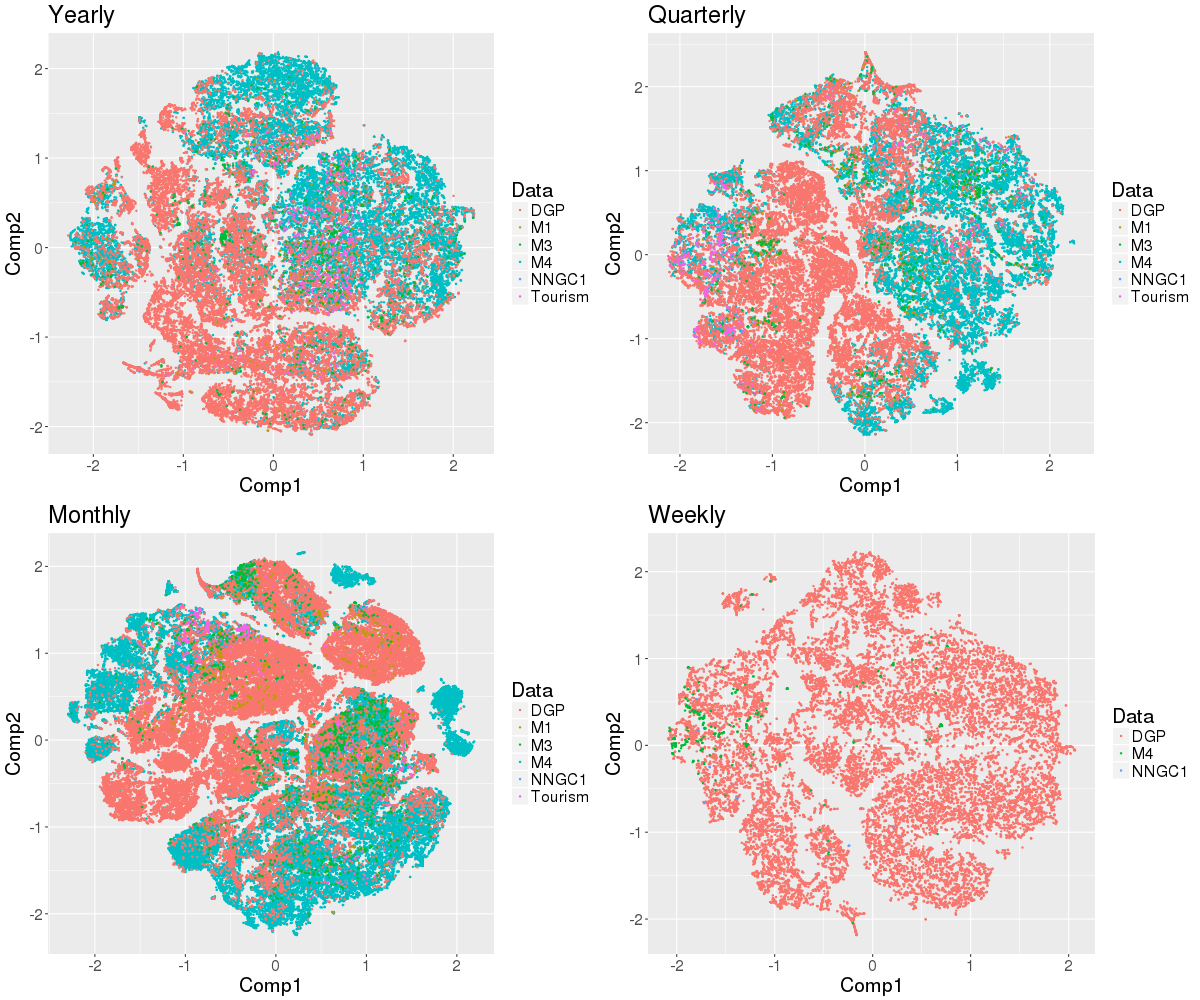
\includegraphics[width=0.9\textwidth]{figures/coverage.png}}

\end{frame}

\begin{frame}{Miscoverage}
\protect\hypertarget{miscoverage}{}

We define the miscoverage of dataset A over dataset B as:

\begin{enumerate}
\tightlist
\item
  Find the maximum ranges of the \(x\) and \(y\) axes reached by the two
  datasets A and B, and cut the \(x\) and \(y\) dimensions into
  \(N_b = 30\) bins.
\item
  In the constructed two-dimensional grid with \(N_b^2 = 900\) subgrids,
  we denote \(\mathcal{I}_{i,A} = 0\) if no points in dataset A fall
  into the \(i\)th subgrid. \(\mathcal{I}_{i,A} = 1\) otherwise. The
  same defination of \(\mathcal{I}_{i,B}\) applies for dataset B.
\item
  The miscoverage of dataset A over dataset B is defined as
  \[\text{miscoverage}_{A/B} = \frac{\sum\limits_{i = 1}^{N_b}[(1 - \mathcal{I}_{i,A})*\mathcal{I}_{i,B}]}{N_b^2}.\]
\end{enumerate}

\end{frame}

\begin{frame}{Miscoverage}
\protect\hypertarget{miscoverage-1}{}

\centerline{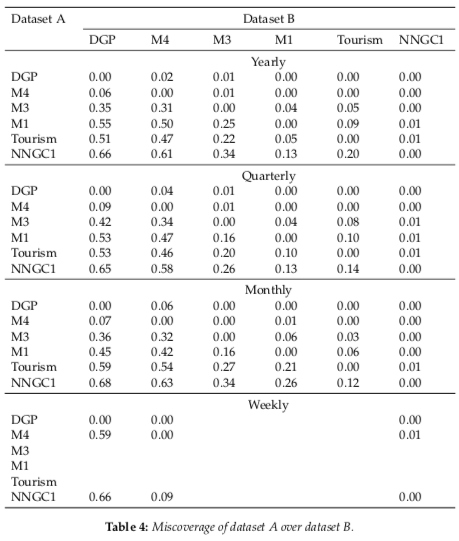
\includegraphics[width=\textwidth]{figures/miscoverage.png}}

\end{frame}

\hypertarget{new-time-series-generation-based-on-mar-models}{%
\section{Efficient time series generation with target features}\label{new-time-series-generation-based-on-mar-models}}

\begin{frame}{Why we do this?}
\protect\hypertarget{new-time-series-generation}{}

\begin{itemize}
  \item 
  Practitioners in certain areas may be only interested in a subset of features.
  \begin{itemize}
    \item
   Heteroskedasticity and volatility in financial time series.
   \item
    Trend and entropy in time series forecasting.
    \item 
    Peaks and spikes in energy time series.
  \end{itemize}
\item
  Therefore, efficient generation of time series with certain features of interest is another important problem to address.
\end{itemize}
\end{frame}

\begin{frame}{How?}
  \begin{itemize}
  \tightlist
  \item
    Genetic Algorithm (GA) to evolve time series with length n
  \item
    GA to tune the MAR model parameters \(\Theta = (\alpha_k, \phi_i)\)
  \end{itemize}


\end{frame}

\begin{frame}{GA procedure}
\protect\hypertarget{ga-procedure}{}

\begin{itemize}
\tightlist
\item
  Firstly decide on the period \(P\) and length \(n\).
\item
  Given a target \(T_i\) in the feature space. Find \(\Theta^{*}\) that
  can simulate \(X_{T_i}\) with its feature vector \(T_i\).
\item
  Generate an initial population of size \(N_P\) for the parameter
  vector \(\Theta\) from the entire possible ranges.
\item
  For each iteration, repeat the steps below.

  \begin{enumerate}
  \tightlist
  \item
    For each member in the current population, simulate a time series
    \(j\) and calculate its feature vector \(F_j\).
  \item
    Calculate the fitness value for each member:
    \[\text{Fitness}(j) = - ||F_j-T_i||.\]
  \item
    Produce the new generation based on the crossover, mutation and the
    survival.
  \end{enumerate}
\item
  Upon convergence, we keep the closest time series.
\end{itemize}

\end{frame}

\begin{frame}{Web application}
\protect\hypertarget{section}{}

\centerline{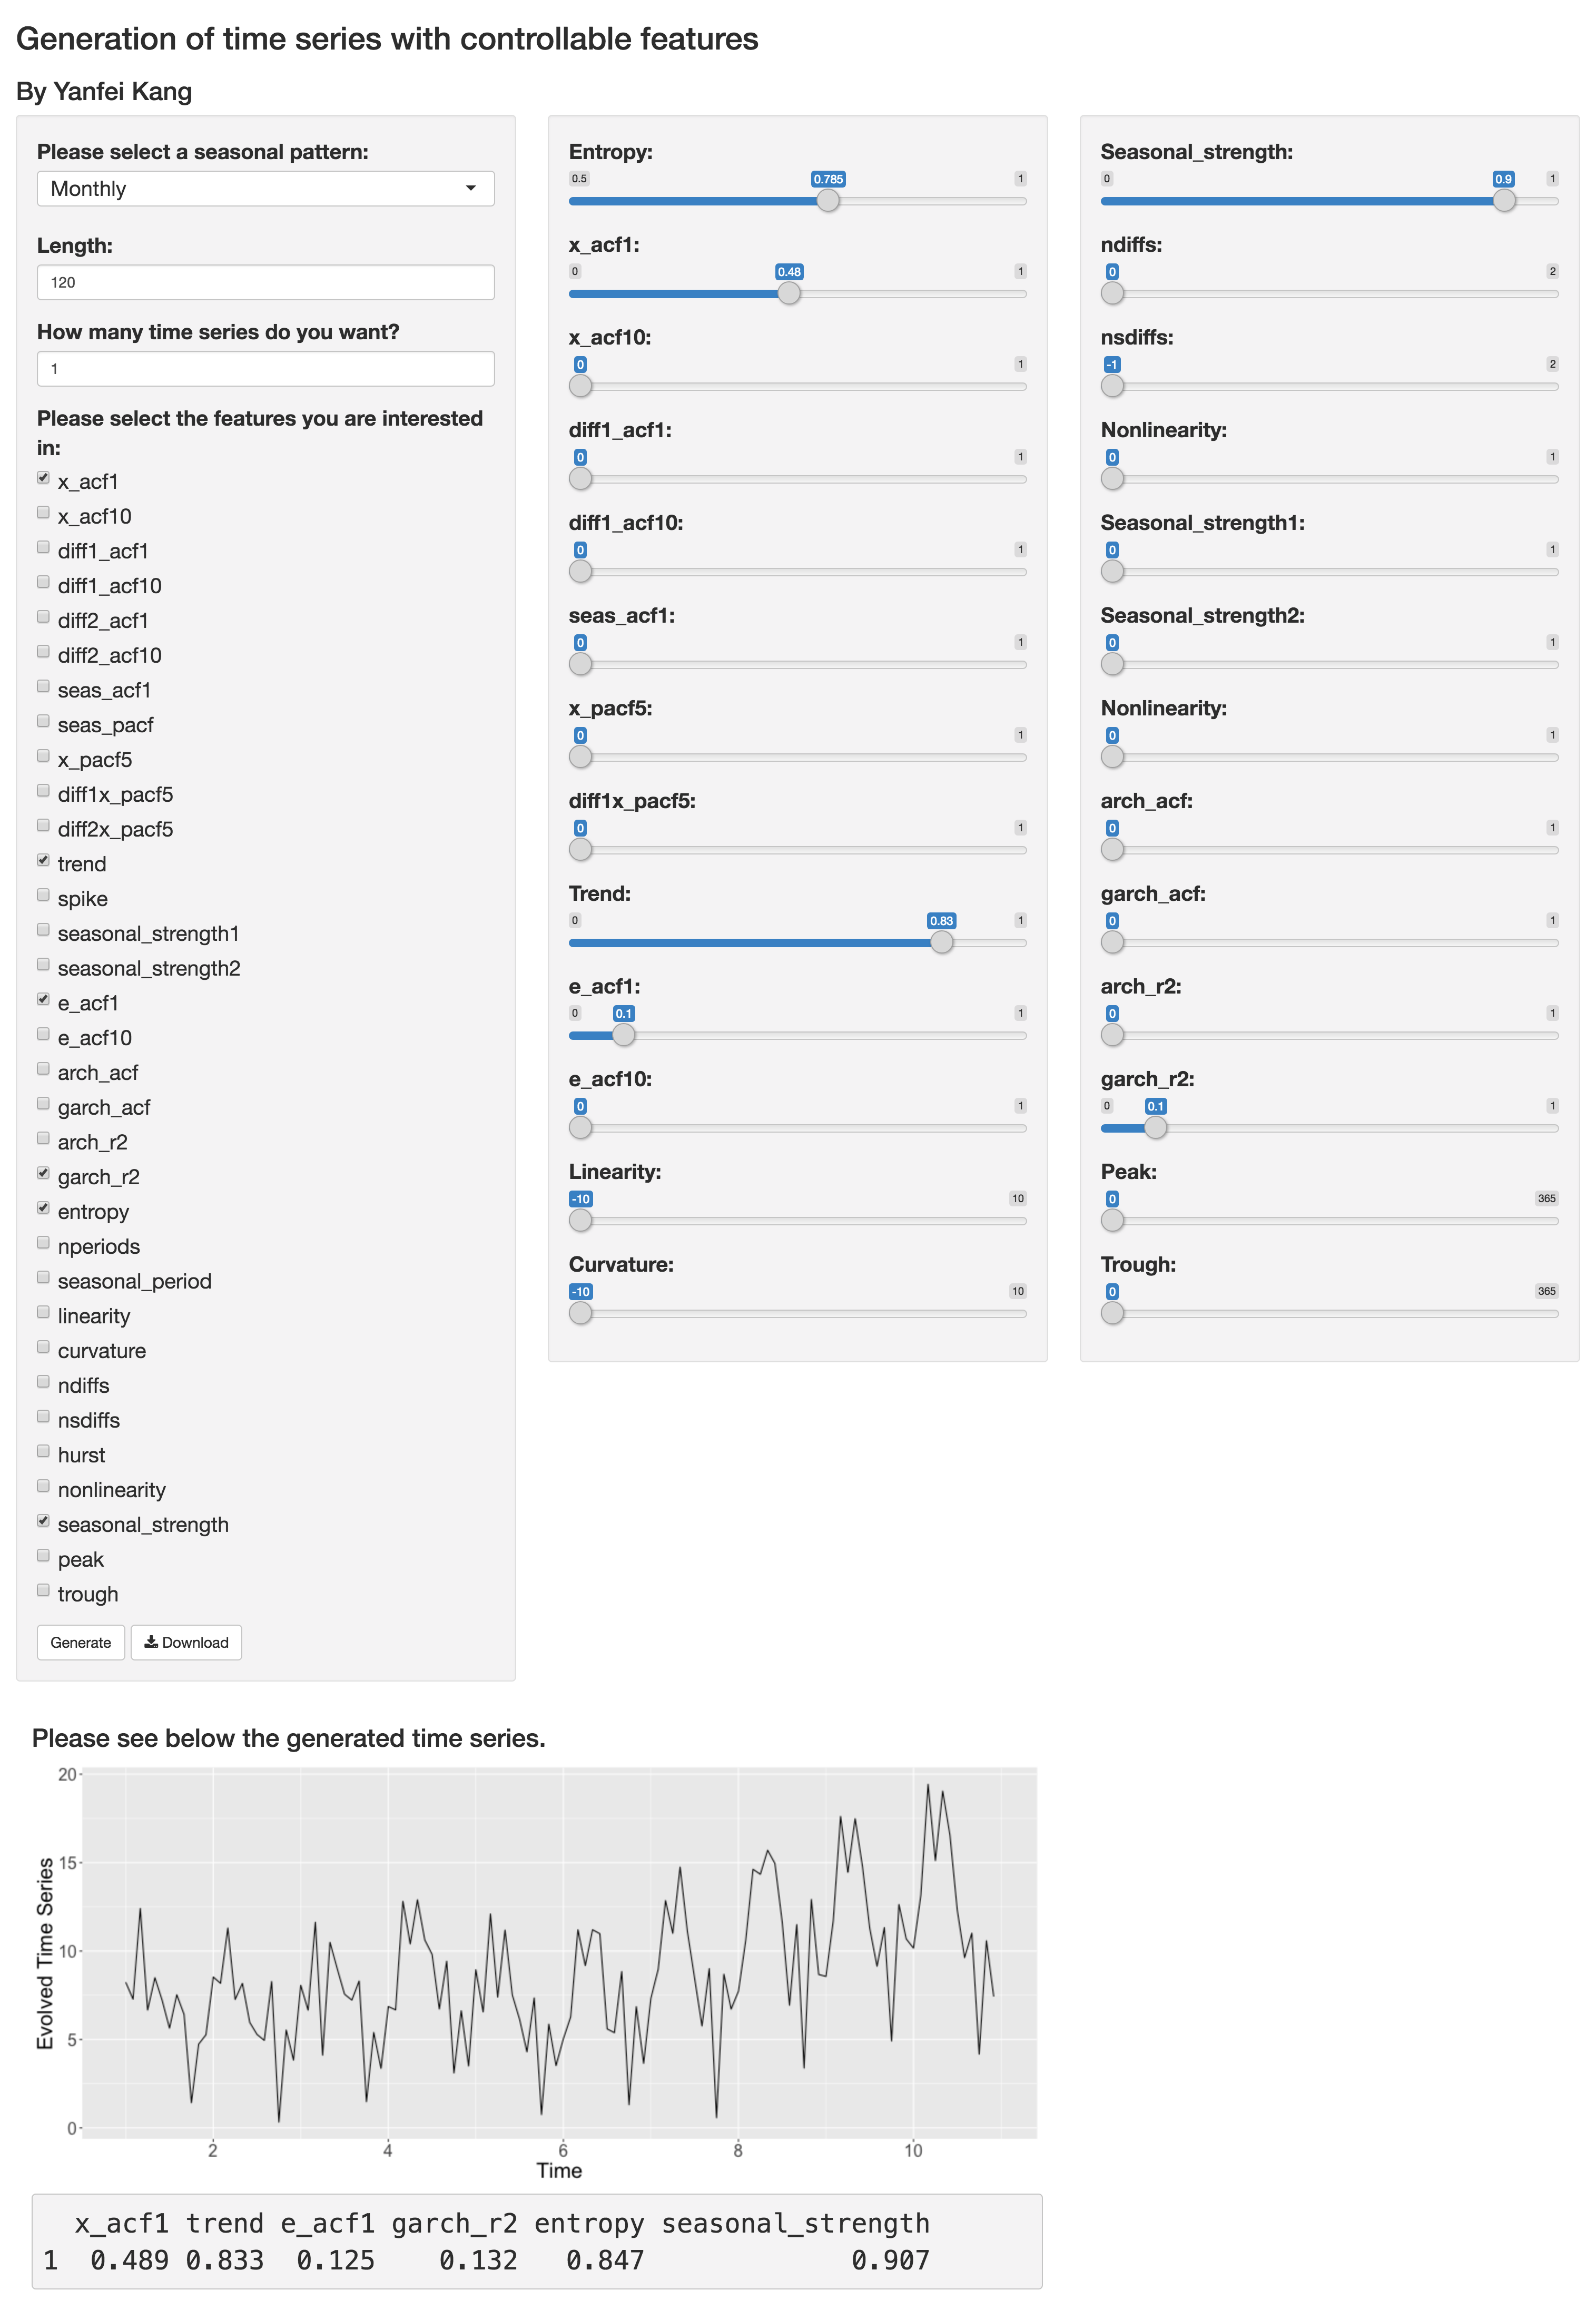
\includegraphics[width=\textwidth]{figures/TSgenerationApp}}

\end{frame}

\hypertarget{forecasting-based-on-features}{%
\section{Application to time series forecasting}\label{forecasting-based-on-features}}

\begin{frame}{The No-Free-Lunch theorem}
\protect\hypertarget{the-no-free-lunch-theorem}{}

\begin{itemize}
\item
  There is never universally best method that fits in all situations
  (Wolpert 1996).
\item
  The explosion of new algorithms development makes the question even
  more worth focusing.
\item
  No single forecasting method stands out the best for any type of time
  series (Adam 1973).
\end{itemize}

\end{frame}


\begin{frame}{Feature-based forecasting}
\protect\hypertarget{literature-1}{}

\begin{itemize}
\item
  Features of time series \(\rightarrow\) benefits in producing more
  accurate forecasting accuracies (Adam 1973)
\item
  Features \(\rightarrow\) forecasting method selection rules (Meade
  2000)
\item
  ``Horses for courses'' \(\rightarrow\) effects of time series features
  to the forecasting performances (Petropoulos et al. 2014)
\item
  Visualize the performances of different
  forecasting methods in a 2D space \(\rightarrow\) better understanding
  of their relative performances (Kang, Hyndman, and Smith-Miles 2017)
\item
  FFORMA \(\rightarrow\) feature-based forecast model averaging (Montero-Manso et al. 2018)
\end{itemize}

\end{frame}

\begin{frame}{Application of GRATIS to M3 data}
\protect\hypertarget{final-aim-forecasting-on-testing-data}{}

\begin{itemize}
\tightlist
\item
  \textbf{Training data}: Randomly generated data via our DGP procedure.
\item
  \textbf{Testing data}: M3 data.
\end{itemize}

\end{frame}

\begin{frame}{Forecasting framework}
\protect\hypertarget{application-to-m3}{}

\centerline{\includegraphics[width=\textwidth]{figures/forecastdiag.pdf}}

\end{frame}

\begin{frame}{Time series features we use}
\protect\hypertarget{time-series-features-we-use}{}

\centerline{\includegraphics[width=0.9\textwidth]{figures/tsfeatures}}

\end{frame}



\begin{frame}{Results}
\protect\hypertarget{results}{}

\centerline{\includegraphics[width=\textwidth]{figures/M3results}}

\end{frame}

\begin{frame}{Conclusions}
\protect\hypertarget{conclusions}{}

\begin{itemize}
\tightlist
\item
  GRATIS for time series generation.
\item
  Benchmarking data.
\item
  The generation is based on MAR models.
\item
  GRATIS can be used for advanced time series analysis.
\item
  We show its usefulness for time series forecasting.
\item
  GRATIS can be used to generated ts with target features.
\end{itemize}

\end{frame}


\begin{frame}{Working paper, R packages and apps}
\protect\hypertarget{r-packages-and-apps}{}

\begin{itemize}
\tightlist
\item
  Yanfei Kang, Rob J Hyndman, Feng Li (2018). GRATIS: GeneRAting TIme
  Series with diverse and controllable characteristics.
  \url{https://arxiv.org/abs/1903.02787}.

\item
  \textbf{R package}: \url{https://github.com/ykang/tsgeneration}.
\item
  \textbf{App}: \url{https://ebsmonash.shinyapps.io/tsgeneration}.
\item
  Special thanks to Mitchell O'Hara-Wild!
\end{itemize}

\end{frame}




\begin{frame}{Thanks!}
\protect\hypertarget{thanks}{}

\Large \url{http://yanfei.site}

\Large \href{mailto:yanfeikang@buaa.edu.cn}{\nolinkurl{yanfeikang@buaa.edu.cn}}

\end{frame}

\end{document}
